Având în vedere limitările tradiționale ale sistemelor HFL, acest studiu propune Învățare Federată Ierarhică Bidirecțională (B-HFL), o familie alternativă de metode care optimizează eficiența datelor și a comunicațiilor. Acest lucru se realizează prin utilizarea structurii ierarhice pentru a organiza comunicarea între servere și pentru a controla diseminarea parametrilor prin următoarele alegeri de design:
\vspace{-0.1cm}
\begin{enumerate}
    \item În timp ce metodele anterioare, cum ar fi HierFAVG~\citep{Client-Edge-CloudHierFL,Hier_Het_Cellular}, înlocuiesc complet modelele edge-server și ale clienților după ce are loc agregarea globală, B-HFL realizează agregarea parțială între un nod copil și părintele său, ceea ce permite copiilor să-și mențină parametrii locali în timp ce încorporează informații globale. Propun modelarea acestei proceduri în două faze:

          \begin{enumerate}
              \item Agregare de la frunze către rădăcină: clienții finalizează antrenamentul, iar informațiile lor sunt propagate înspre rădăcina arborelui. Fiecare nod intern are un parametru $T_n$, care determină după câte runde trimite actualizările către părinte. Această valoare este echivalentă cu epocile locale ale clientului și poate fi: aceeași pentru toate nodurile, aceeași pentru toate nodurile de la un anumit nivel al arborelui sau setată independent pentru fiecare nod.
              \item Agregare de la rădăcină către frunze: După ce un nod a primit și a agregat rezultatul antrenamentului de la unii sau toți copiii săi, își propagă parametrii în josul subarborelui său. Costul acestei propagări este proporțional cu adâncimea subarborelui. Cu toate acestea, conexiunea dintre nodurile interne este mai rapidă decât cea a clienților către serverele edge.
          \end{enumerate}
    \item Nodurile interne din cadrul structurii ierarhice pot fi antrenate pe seturi de date proxy pentru regularizarea antrenamentului~\citep{OneShotFL,FLwithNonIID}. Antrenamentul proxy este în mod special relevant pentru modelarea limbajului, deoarece sunt disponibile corpuri textuale publice de dimensiuni considerabile. Pentru a evita operarea pe parametrii învechiți, momentul natural pentru a adăuga un astfel de antrenament este imediat după ce agregarea de la frunză către rădăcină ajunge la nod. Cu toate acestea, latența rezultată dintr-un astfel de antrenament poate fi prea mare. În acest caz, antrenamentul poate utiliza asincron parametrii învechiți în timp ce subarborii nodului se execută.
    \item Toate nodurile pot fi lăsate să funcționeze sincron sau asincron în ceea ce privește alte noduri de pe același nivel, dacă este necesar, în timpul agregării de la frunze către rădăcină. Pentru frunzele (clienții) sub controlul unui server edge, acest lucru este echivalent cu FL asincron tradițional~\citep{AsynchronousFLonHetDevicesSurvey}. Pentru un nod intern, aceleași strategii federate asincrone~\citep{FedBuff,PAPAYA} pot fi aplicate atunci când primesc modele de la nodurile copil, execuția clientului fiind înlocuită de execuția subarborelui.
\end{enumerate}

Parametrii agregați de la nodurile frunze (clienți) prin arbore sunt antrenați fin la datele locale relevante. În contrast, parametrii transmiși de la părinți la copii sunt agregați peste populații mai numeroase. Când serverele cuprind clienți grupați semnificativ, aceste populații numeroase pot fi mai puțin legate (de exemplu, conținând mai multe limbi). În plus, dacă nodurile interne sunt lăsate să se antreneze pe seturi de date proxy, ele injectează antrenament suplimentar în modelele federate și oferă regularizare pentru întregul arbore. În abordările FL tradiționale, antrenamentul pe serverul care controlează direct clienții poate impune o regularizare prea puternică. Totuși, în B-HFL, nodurile superioare din arbore reprezintă deja o imagine globală și au un impact limitat asupra frunzelor, deoarece influența lor se diluează prin intermediul mai multor noduri intermediare. În final, clienții sunt tratați omogen cu orice alt nod, deoarece mențin un model persistent local pe parcursul rundelor și fiecare client este agregat doar parțial cu părintele.

Deoarece nu toate nodurile din arbore sunt obligate să fie capabile de antrenament, merită distinse modelele care au fost optimizate prin antrenare suplimentară, în loc de simplă agregare. În mod specific, disponibilitatea datelor de antrenament poate permite metode de agregare mai eficiente, cum ar fi învățarea mutuală~\citep{DeepMutualLearning} sau regularizarea bazată pe $l_2$~\citep{Ditto}. În plus, actualizările construite prin antrenament direct pot oferi un semnal de optimizare mai bun. Astfel, această lucrare propune adăugarea de fluxuri de date directe între nodurile capabile de antrenament (de exemplu, clienți și rădăcină) în timp ce se folosește structura de comunicare ierarhică subiacentă, ca o conexiune reziduală în ResNet~\citep{ResNet}. De exemplu, sistemul ar putea permite ca actualizările cu cea mai mare valoare absolută a $K$ clienți de la fiecare server să fie transmise către rădacină, unde ele pot fi unite fie prin antrenament, fie prin optimizare adaptivă. Acest tip de conexiune verticală oferă un flux de date foarte dinamic și potențial ciclic. O altă cale ce merită explorată este permiterea nodurilor, în special a clienților, de a se antrena în mod asincron folosindu-și modelul persistent. Acest lucru ar permite clienților să țină cont de schimbarea setului de date local, folosind tehnici bine-cunoscute din literatura privind învățarea continuă~\citep{ContinualLearningSurvey,kirkpatrick2017overcoming}. Sistemul poate aduce multiple beneficii potențiale:
\begin{enumerate}
    \item Poate găzdui noduri care au metode diferite de agregare, rate de învățare, stări dinamice ale optimizatorului pentru agregarea de la frunză către rădăcină și de la rădăcină către frunză. În mod similar numărului de runde $T$, parametrii legați de agregare pot fi independenți sau omogeni.
    \item Grupurile mai mici pentru fiecare server edge evită problema scăderii mărimii pseudo-gradientului~\citep{LargeCohorts}. Un efect similar este generat de clusterizarea clienților pentru serverele edge.
    \item În timp ce modelele locale persistente sunt cunoscute pentru funcționarea lor eficientă în FL cross-silo, această structură ierarhică le face relevante în setările cross-device prin posibilitatea de a selecta un număr mai mare de clienți, permițându-le să fie vizitați în mod repetat.
    \item Poate integra în mod natural Secure Aggregation~(SecAgg)~\citep{SecAggOG} la nivelul fiecărui server edge. Precum menționat de \citet{ScaleSystemDesign}, ierarhizarea reduce costul de comunicare suplimentar al antrenării a $C$ clienți cu SecAgg de la $\mathcal{O}(C^2)$ la $\mathcal{O}(C^2/M)$ unde M este numărul de servere edge.

\end{enumerate}

\subsection{Exemplu de sistem}\label{sec:example_system}
\begin{figure}[h]
    \centering
    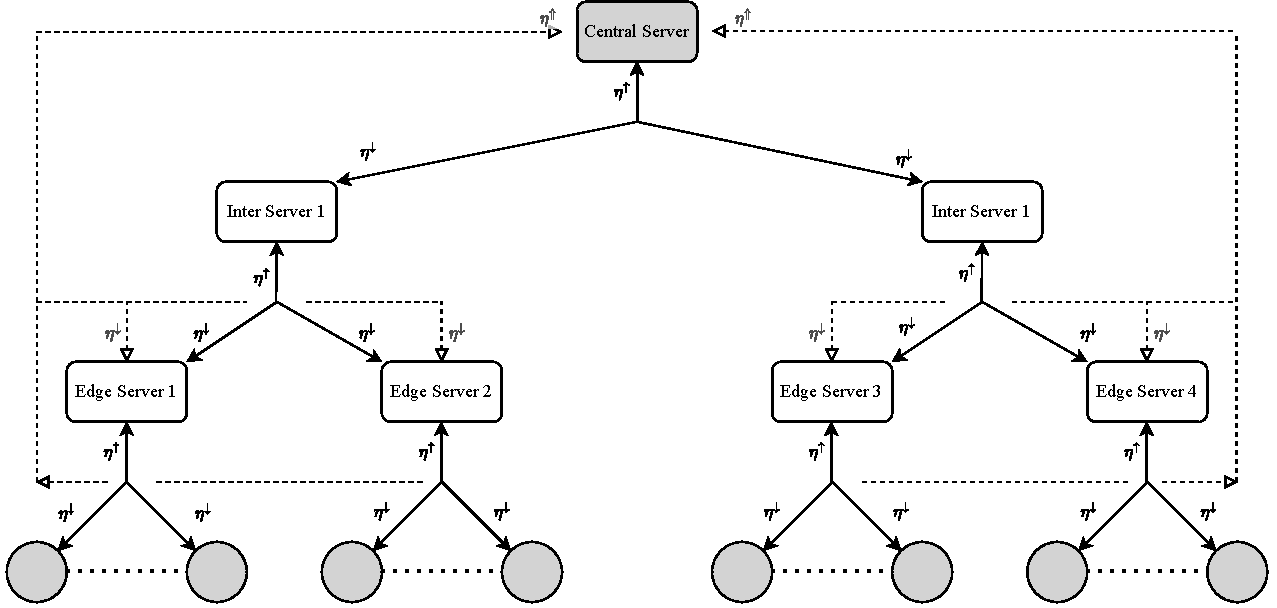
\includegraphics[clip,width=.8\columnwidth]{plots/Tree_Structure.drawio.pdf}
    \caption[System Diagram]{Diagramă a unui exemplu de sistem B-HFL. Liniile solide reprezintă legături de comunicare, în timp ce liniile punctate reprezintă conexiuni "reziduale" conceptuale, folosind legăturile de bază. Nodurile capabile de antrenament, cum ar fi clienții sau serverul central cu un set de date proxy, sunt în gri. Când parametrii modelului se propagă în sus, nodurile combină pseudo-gradienții de intrare și își actualizează modelul, folosind rata de învățare de la frunză către rădăcină $\eta^\uparrow$. La fel se întâmplă când parametrii curg de la nodurile părinte către nodurile copil cu rata de învățare $\eta^\downarrow$. Deoarece liniile punctate comunică de la $0$ la $K$ modele, $\eta^\Uparrow$ poate reprezenta de la $0$ la $K$ agregări, folosind o rată de învățare $\eta^\uparrow$.
    }\label{fig:TreeStructure}
\end{figure}

Un exemplu de sistem B-HFL, care ar fi principalul rezultat al acestei propuneri, poate fi văzut în \cref{fig:TreeStructure}. Serverul central controlează un set de date proxy folosit pentru antrenament post-agregare. Toate serverele își trimit actualizările către părinte după fiecare runda. Fiecare nod, inclusiv clienții, rulează cel puțin două optimizatoare FedOPT cu stări separate și rate de învățare, una pentru agregarea de la frunză către rădăcină cu pseudo-gradientul mediu $\Delta_t$ și una pentru agregarea părinților. Chiar dacă aceeași rată de învățare de la frunză la rădăcină $\eta^\uparrow$ și rata de învățare de la rădăcină la frunză $\eta^\downarrow$ ar fi utilizate pentru toate nodurile, stările independente ale optimizatorului serverului ar distinge procedura de agregare a nodului.

Conexiunile reziduale îndeplinesc funcții diferite între etapele de la frunză la rădăcină și de la rădăcină la frunză. Pentru etapa ascendentă, ele colectează actualizarea clientului cu valoarea absolută cea mai mare de la toate serverele edge, trimițând astfel un model suplimentar la serverul central pentru fiecare server edge. Serverul central poate apoi menține stări independente ale optimizatorului pentru fiecare conexiune "reziduală" de intrare. Pentru etapa descendentă, ele oferă serverelor edge șansa de a beneficia direct de antrenamentul serverului central fără a fi nevoie să se bazeze pe modelele diluate ale celor intermediare.

